\documentclass{beamer}

\usepackage{graphicx}
\usepackage{listings}
\usepackage[
	backend=biber,
	style=verbose,
	sorting=ynt
]{biblatex}

\usepackage{derivative}
\usepackage{subfig}
\usepackage{tikz}
\usepackage{pgfplots}
\pgfplotsset{compat=1.18}

\addbibresource{references.bib}

\usetheme{cs}


% Document data for the title page
\title{Galerkine methods for the 1D Helmholtz equation}
\subtitle{An introductory example}
\author[V.~de Nodrest]{V.~de Nodrest\inst{1}}
\institute[UFT/VFU]{
  \inst{1} CentraleSupélec, Université Paris Saclay
}
\date{\today}


% Definir o nome do orientador
\newcommand{\advisorname}{\textbf{Orientador:}  Prof. Dr. Nome do Orientador}


% The next block of commands puts the table of contents at the beginning of each section and highlights the current section
\AtBeginSection[]
{
  \begin{frame}
    \frametitle{Table of Contents}
    \tableofcontents[currentsection]
  \end{frame}
}


\begin{document}


\titlegraphic{\logocstext \hspace{2em} \logogretext}

\frame{\titlepage}

% Insert the general toc
\begin{frame}{Table of Contents}
  \tableofcontents    
\end{frame}

\section{First}

\subsection{First first}


\begin{frame}
  \frametitle{The Helmholtz equation}

  Bla
\end{frame}


\begin{frame}[fragile]
  \frametitle{Our problem}

  We will consider the following complex-valued problem:

  \begin{block}{Our 1D Helmholtz problem}
    \vspace{-0.6cm}
    \begin{align*}
      \odv[2]{u}{x} + k^2 u &= 0 ~ ~ {\text in} ~ ~ ]0, 1[ \\
      u(0) &= i k \\
      u(1) &= i k u(1)
    \end{align*}
    \vspace{-0.6cm}
  \end{block}

\end{frame}


\begin{frame}
  \frametitle{The exact solution}

  The problem can be solved
  by seperating the real and imaginary parts
  and using first year real analysis results
  (linear partial differential equations of order 2).
  This yields the unique solution thus defined:

  \begin{block}{The exact solution}
    \vspace{-0.6cm}
    \begin{align*}
      \forall x \in [0, 1], ~ u(x) &= e^{ikx} 
    \end{align*}
    \vspace{-0.6cm}
  \end{block}

  \begin{figure}
    \centering
    \subfloat[First subfigure\label{fig:a}]{

      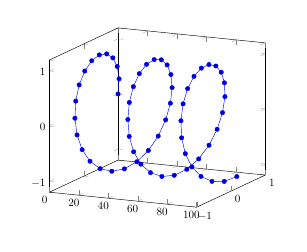
\begin{tikzpicture}[scale=0.4]
        \begin{axis}[view={25}{15}]
            \addplot3+ [
                domain=0:100,
                samples=60,
                samples y=1,
            ] (
        {x},
        {cos(10*\x)},
        {sin(10*\x)}
        );
        \end{axis}
      \end{tikzpicture}
    }
    \qquad
    \subfloat[Second subfigure\label{fig:b}]{
      \begin{tikzpicture}[scale=0.7]
      \draw (0,0) -- (1,1) plot coordinates {(2,0)  (4,0)};
      \draw[color=red,xshift=5cm]
            (0,0) -- (1,1) -- plot coordinates {(2,0)  (4,0)};
    \end{tikzpicture}
    }
  \caption{A figure}
  \label{fig:1}
  \end{figure}

\end{frame}





\begin{frame}[fragile]
  \frametitle{A beamer style for CS x Greenwich}
  
  \begin{block}{Getting started}
    \begin{verbatim}
\documentclass{beamer}
\usetheme{cs}
    \end{verbatim}
  \end{block}
  
  \begin{block}{Commands}

	  \begin{itemize}

      \item \verb|\logocstext[<scale>]| \\
            displaying the CentraleSupélec logo with text\\
			\centerline{\logocstext}

      \item The logo is scaled to fixed height

      \item \verb|\timestamp| \\
            displaying compilation date\\
            \centerline{\timestamp}
        
	  \end{itemize}

  \end{block}
  
\end{frame}


\begin{frame}[fragile]

    \frametitle{A title...}
    \framesubtitle{And a subtitle!}
    
    \begin{block}{Commands}
      \begin{itemize}
      
        \item \verb|\logogretext[<scale>]| \\
              displaying the University of Greenwich's logo with text\\
        \centerline{\logogretext}
        \item The logo is scaled to fixed height
      \end{itemize}
    \end{block}
    
\end{frame}


\section{Example Slides}


\begin{frame}[plain]
  
  \begin{block}{Plain frame}
    This feels empty...
  \end{block}
  
\end{frame}

\begin{frame}{Example slide 0}
  \begin{block}{Block}
      Sample text in a normal block. \alert{Alerted text.}
  \end{block}

  \begin{alertblock}{Alert block}
      Sample text in an alert block
  \end{alertblock}    
  
   \begin{example}
      Sample text for an example
  \end{example}
\end{frame}


\begin{frame}{Example slide 1}
  We compute the matrix of outputs as\footnote{\cite{vaswaniAttentionAllYou2023}}:
  $$
    \mathrm{Attention}(Q, K, V) = \mathrm{softmax}(\frac{QK^T}{\sqrt{d_k}})V
  $$
\end{frame}
  
\begin{frame}{Example slide 2}
  \begin{table}
    \centering
    \begin{tabular}{|c|c|c|}
    \hline
    \textbf{Header 1} & \textbf{Header 2} & \textbf{Header 3} \\
    \hline
    Cell 1-1 & Cell 1-2 & Cell 1-3 \\
    \hline
    Cell 2-1 & Cell 2-2 & Cell 2-3 \\
    \hline
    Cell 3-1 & Cell 3-2 & Cell 3-3 \\
    \hline
    \end{tabular}
    \caption{A Simple Table}
  \end{table}
\end{frame}
  
\section{Bibliography}
  
  \begin{frame}[t,allowframebreaks]
  \frametitle{Bibliography}
  \printbibliography
\end{frame}

\end{document}